\section{Zielsetzung}
\label{sec:ziel}
Das Geiger-Müller-Zählrohr ist ein in der Kernphysik zur Messung ionisierender Strahlung verwendetes Messgerät. Im folgenden Versuch sollen Aufbau 
und Wirkunsgweise verstanden und Charakteristika des Zählrohres untersucht werden.

\section{Theorie}
\label{sec:Theorie}

Bevor das Geiger-Müller-Zählrohr beschrieben und erläutert wird, wird zunächst auf ionisierende Strahlung eingegangen.
Als ionisierende Strahlung wird sowohl Teilchen-, als auch elektromagnetische Strahlung bezeichnet, die aus anderen Atomen und Molekülen Elektronen entfernen können.
In dem folgenden Versuch wird ioniesierende $\beta$-Strahlung betrachtet, die von Thallium emittiert wird.
Ionisierende Strahlung kann für den menschlichen Körper gesundheitliche Schäden verursachen, weshalb es wichtig ist die drei A-Regeln zu beachten, um das Risiko so gut wie möglich zu verringern.
Die drei A-Regeln lauten wie folgt,
\begin{enumerate}
    \item Abstand zum strahlenden Stoff vergrößern.
    \item Aussetzungszeit, also die Kontaktzeit zum Stoff, verringern.
    \item Abschirmen, sodass die Strahlung möglichst viel Materie durchdringen muss, um sie weitesgehend abzuschwächen.
\end{enumerate}

Ein Geiger-Müller-Zählrohr besteht aus einem Kathodenzylinder mit dem Radius $r_{\text K}$ mit einem darin axial verlaufenden Anodendraht mit dem Radius $r_{\text A}$.
Wenn eine äußere Spannung angelegt wird, so entsteht ein radialsymmetrisches Feld zwischen der Kathode und der Anode.
Das Feld hat die Feldstärke
\begin{align}
    E(r)=\frac{U}{\rho\ln(\sfrac{r_{\text K}}{r_{\text A}})},
\end{align}
wobei $\rho$ der Abstand von der Zählrohrachse ist.
Die Beschleunigung, die ein Teilchen in dem Radialfeld erfährt ist beliebieg groß, wenn $r_{\text A}$ klein genug gewählt wird. \newline
Die Zylinderkathode ist mit einem Gas, wie zum Beispiel $\SI{100}{\milli\bar}$ Argon und $\SI{10}{\milli\bar}$ Ethylalkohol, gefüllt. Dringt ein geladenes Teilchen
in das Zählrohrvolumen ein, so bewegt es sich solange durch den Gasraum, bis die Energie des Teilchens volltständig durch Ionisationsakte aufgebraucht wird. Die Anzahl
der in diesem Prozess entstehenden Elektronen ist dabei proportional zur Energie des einfallenden Teilchens.
In \autoref{fig:schemGeiger} ist der schematische Aufbau eines Geiger-Müller-Zählrohres abgebildet.
\begin{figure}[H]
    \centering
    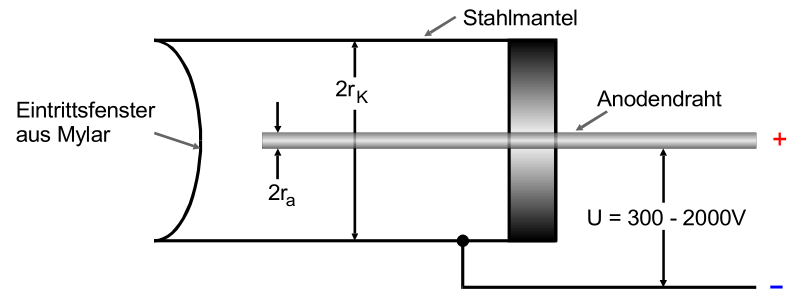
\includegraphics[width=0.7\textwidth]{data/zaehlrohr.png}
    \caption{Schematische Darstellung eines Geiger-Müller-Zählrohres.}
    \label{fig:schemGeiger}
\end{figure}

Die im Zählrohr ablaufenden Vorgänge sind stark abhängig von der im Zylindermantel angelegten Spannung.

\subsection{Teilbereiche eines Zählrohres}
\label{subsec:TheoVerlauf}

Eine Darstellung der Anzahl emittierten Elektronen ist in \autoref{fig:verlauf} gegenüber der angelegten Spannung in einem Proportionalzählrohr abgebildet.
Es werden fünf verschiedene Teilbereiche unterschieden, die im folgenden näher erläutert werden sollen.
\begin{figure}[H]
    \centering
    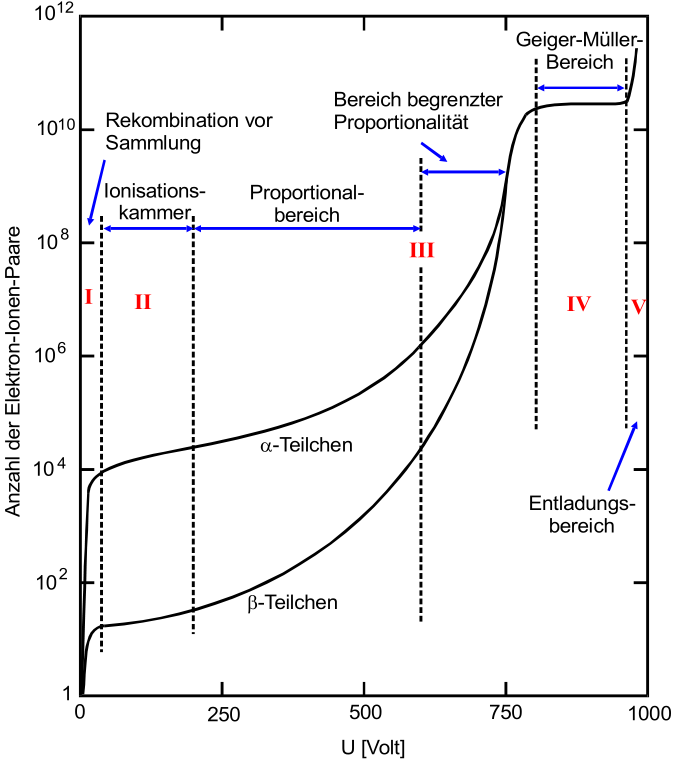
\includegraphics[width=0.5\textwidth]{data/verlauf.png}
    \caption{Anzahl der erzeugten Elektronen in Abhängigkeit der angelegten Spannung $U$.}
    \label{fig:verlauf}
\end{figure}

Der erste Teilbereich ist der Bereich, in dem nur ein Teil der erzeugten Elektronen den Draht erreicht, da eine zu kleine Spannung $U$ angelegt ist 
und der Rest durch Rekombination verloren geht. \newline
Die Rekombinationswahrscheinlichkeit sinkt bei einer höheren Betriebsspannung $U$, denn es erreichen fast alle Elektronen den Anodendraht. 
Der kontinuierlich fließende Ionisationsstrom ist in diesem Bereich proportional zur Energie und zu der Intensität der einfallenden Strahlung. Ein Gerät,
das unter ebendiesen Bedingungen arbeitet, stellt eine Vorstufe zu einem Zählrohr dar und wird Ionisationskammer genannt. Weil die Ionisationsströme nur sehr gering sind, kann so ein Gerät nur bei
hohen Strahlungsintensitäten eingesetzt werden. \newline
Wird die Feldstärke weiter erhöht, so erreicht sie in Drahtnähe so hohe Werte, dass die emittierten Elektronen zwischen den Zusammenstößen mit den Argon-Atomen so viel Energie besitzen, um selber Ionisation zu erzeugen.
Dieser Vorgang wird Stoßionisation genannt. Durch die von den Elektronen hervorgerufene Ionisation werden weitere Elektronen emittiert und es kommt zu einem lawinenartigen Anstieg ihrer Anzahl, was als Townsend-Lawine beizeichnet wird. 
Die pro einfallendes Teilchen am Zählrohrdraht gesammelte Ladung $Q$ ist in diesem Teilbereich so groß, dass sie als Ladungsimpuls gemessen werden kann. Dieser Ladungsimpuls kann, aufgrund der weiterhin vorliegenden Proportionalität zwischen Ladung und Energie,
als Maß für die Teilchenenergie genommen werden. Es ist in diesem Strahlungsbereich also möglich neben der Strahlungsintensität auch die Teilchenenergie zu messen. Aufgrund der erwähnten Proportionalität werden Geräte, die in diesem Teilbereich arbeiten als Proportionalzählrohre bezeichnet. \newline
Wird die Betriebsspannung $U$ weiter erhöht, so wird die Ladung $Q$ unabhängig von der Primärionisation. Deshalb wird dieser Bereich auch Auslösebereich genannt. In diesem Bereich arbeitet das Geiger-Müller-Zählrohr.
Die Entladung beschränkt sich in diesem Bereich nicht nur auf lokalisierte Elektronenlawinen, die sich nur in Feldrichtung ausbreiten, sondern breiten sich auch längs des gesamten Zählrohrdrahtes aus.
In der primären Elektronenlawine entstehene UV-Photonen durch die Anregung der Argon-Atome durch Elektronenstöße. Diese UV-Photonen wiederum erzeugen durch Ionisation weitere freie Elektronen. Weil Photonen elektrisch neutral geladen sind, können sie sich auch senktrecht zum elektrischen Feld ausbreiten
und erzeugen deshalb im gesamten Zylinder neue Elektronenlawinen. Die am Zählrohr  gesammelte Ladung hängt nur noch vom Volumen des Zählrohres und der Höhe der Betriebsspannung ab, weshalb das Zählrohr nur noch zur Intensitätsmessung benutzt werden kann.
Der Auslösebereich beginnt in \autoref{fig:verlauf} dort an, wo die $\alpha$- und $\beta$-Kurven ineinander übergehen. Dort ist der Ladungsimpuls am Ausgang des Zählrohres unabhängig vom Ionisationsvermögen der einfallenden Strahlung.

\subsection{Einfluss der positiven Ionen auf die Verlaufskurve}
\label{subsec:posIon}

Die beim Entladevorgang entstehenden Elektronen bewegen sich relativ schnell zum Draht. Die positiv geladenen Ionen halten sich allerdings länger im Gasraum auf, weil sie eine wesentlich größere Masse besitzen. Die positiven Ionen bauen vorübergehend
eine radialsymmetrische, positive Raumladung, den Ionenschlauch, auf. Das setzt die Feldstärke des Drahtes für eine gewisse Zeit herab und es findet praktisch keine Stoßionisation mehr satt. Während dieser Zeit werden keine eintreffenden Teilchen vom Zählrohr detektiert,
weshalb man diesen Zeitraum auch als Totzeit $T$ bezeichnet. Nachdem die positiven Ladungen abgewandert sind erreichen die abgegebenen Ladungsimpulse aber ers ihr ursprüngliches Maximum, wenn die positiven Ionen vollständig neutralisiert sind.
Deshalb folgt auf die Totzeit $T$ eine weitere Zeit, in dem die Ausgangsimpulse eine geringere Höhe haben, die Erholzeit $T_{\text T}$. Eine schematische Darstellung der Tot- und Erholzeit sind in \autoref{fig:totzeiten} dargestell.
\begin{figure}[H]
    \centering
    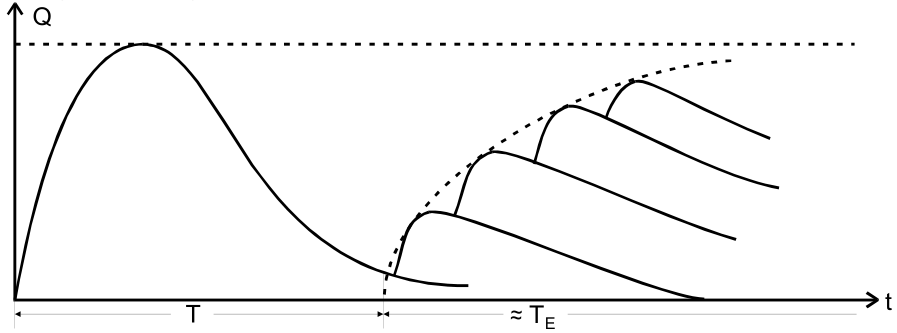
\includegraphics[width=0.5\textwidth]{data/totzeiten.png}
    \caption{Schematische Darstellung der Tot- und Erholzeiten.}
    \label{fig:totzeiten}
\end{figure}

Auftreffende Ionen auf dem Zählrohrmantel können Elektronen aus der Metalloberfläche herauslösen, weil die bei der Neutralisation freigesetzte Energie groß genug ist, um die Austrittsarbeit für Elektronen zu überwinden.
Elektronen, die aus der Metalloberfläche gelöst werden, werden Sekundärelektronen genannt. Sie durchlaufen das gesamte Zählrohrpotential durch und können deshalb erneute Zählrohrentladungen entzünden. Nach dem Durchgang eines einzelnen Teilchens 
durch das Gasvolumen, entstehen also mehrere, zeitlich versetzte Ausgangsimpulse, die als Nachentladungen bezeichnet werden. Ihr zeitlicher Ablauf $T_{\text L}$ ist größer, als die Totzeit $T$ und ist deshalb höchst unerwünscht.
Um die Nachentladungen möglichst gering zu halten, wird zum Zählrohrgas zusätzlich ein Anteil von Alkoholdämpfen hinzugefügt. Die Ionen stoßen mit den Alkoholmolekülen zusammen. Diese werden aufgrunde einer geringeren Ionisierungsenrgie ioniesiert und wandern zur Kathode und werden dort neutralisiert.
Die Energie, die dabei freigesetzt wird, reicht nicht mehr für die Emission von Elektronen aus und wird zur Anregung von Schwingungen der Alkoholmoleküle verwendet. Das Zählrohr wird somit nur noch durch neu einfallende Teilchen ausgelöst.

\subsection{Charakteristik des Zählrohres}
\label{subsec:ZaehlrohrCharakteristik}

Wird die Anzahl der im Geiger-Müller-Zählrohr eintreffenden Teilchen $N$ bei einer konstanten Strahlungsintensität gegen die angelegte Betriebsspannung $U$ angelegt, so erfolgt die in \autoref{fig:charakteristik} abgebildete schematische Darstellung.
\begin{figure}[H]
    \centering
    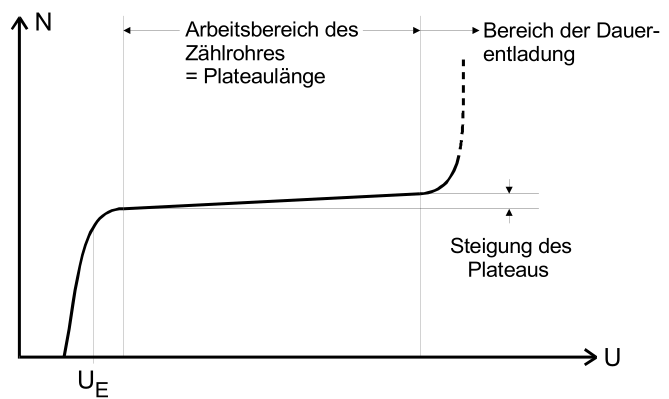
\includegraphics[width=0.5\textwidth]{data/charakteristik.png}
    \caption{Schematische Darstellung der Zählrohrcharakteristik bei konstanter Strahlungsintensität.}
    \label{fig:charakteristik}
\end{figure}

Ungefähr ab der Spannung $U_\text E$ fängt der Auslösebereich des Zählrohres an. Bei höherer Betriebsspannung setzt ein linearer Teil ein, der Plateau genannt wird. Bei einem idealen Zählrohr wäre die Plateausteigung null, in der Praxis ist aber immer eine geringe Spannung zu erkennen.
Das liegt vor allem daran, dass einige Nachladungen, trotz des Zusatzes der Alkoholanteile, noch entstehen. Das Plateau ist ein Indikaor für die Qualität des Zählrohres, denn je geringer die Steigung und je länger das Plateau, desto höher ist die Qualität des Zählrohres.
Das Ende des Plateau geht in den Bereich der selbstständigen Ladung über Gasentladung über, in der im Zählrohr durch ein einzelnes Teilchen eine Dauerentladung entsteht. Das Zählrohr kann in diesem Bereich aufgrund der hohen Spannungsansteigungen schnell zerstört werden.
Der besprochene Bereich ist in \autoref{fig:verlauf} im fünften Abschnitt eingetragen.

\subsection{Ansprechvermögen des Zählrohres}
\label{subsec:Ansprechvermoegen}

Als Ansprechvermögen des Zählrohres wird die Wahrscheinlichkeit bezeichnet ein einfallendes Teilchen im Zählrohr nachzuweisen. Bei $\alpha$- und $\beta$-Strahlung liegt das Ansprechvermögen, wegen ihres hohehn Ionisationsvermögen, bei nahzeu $100\%$.
Wegen der hohen Wechselwirkung mit Materie wird diese Art von Strahlung im Zählrohrmantel vollständig absorbiert. Es muss also garantiert werden, dass die Strahlung überhaupt erst in das Zählrohr gelangt. Dazu werden Endfensterzählrohre, deren Stirnseite aus einem
Material mit niedriger Ordnungszahl besteht, verbaut. Diese auch als Mylar-Folie bezeichnete Öffnung ermöglicht es, dass selbst $\alpha$-Teilchen hindurchgehen können. Durch den Unterdruck im Zählrohr ist die Folie nach innen gekrümmt. \newline
Das Ansprechvermögen für Photonen ist wegen der geringen Wechselwirkung eher gering und liegt bei hochenergetischer Photonenstrhlung bei ungefähr $1\%$. Geiger-Müller-Zählrohre eignen sich also nur bei hochenergetischer $\gamma$-Strahlun und bei niederenergetischen Röntgenstrahlen, die vor allem bei schweren Füllgaselementen
wie Xenon gut messbar sind.